\newif\ifRELEASE
%\RELEASEfalse
\RELEASEtrue

\documentclass[10pt,handout]{beamer}

\usepackage{amsmath,amssymb,enumerate,calc,color,ifthen,capt-of,booktabs,graphicx,listings,palatino,amsbsy,subfigure, tikz}

%\usetikzlibrary{calc}
\usetikzlibrary{shapes}

\usefonttheme{serif}
 
\definecolor{light-gray}{gray}{0.95}
\lstset{basicstyle=\footnotesize\ttfamily,
        %numbers=left,
        %backgroundcolor=\color{light-gray},
        frame=single, 
        %rulesepcolor=\color{red},
        keywordstyle=\color[rgb]{0,0,1},
        commentstyle=\color[rgb]{0.133,0.545,0.133},
        stringstyle=\color[rgb]{0.627,0.126,0.941},
        captionpos=b,
        title=\lstname,
        showstringspaces=false
       }


%---TITLE AND AUTHOR INFORMATION
\title % (optional, use only with long paper titles)
[MPI in Python]{Introduction to MPI using {\tt mpi4py}}
\author[Roberts]{Prof.~Jeremy Roberts}
% \institute[22.213] % (optional, but mostly needed)
%  {}
% - Keep it simple, no one is interested in your street address.
\date
%[CFP 2003] % (optional, should be abbreviation of conference name)
{Fall 2015}


\begin{document}

% TITLE PAGE
\begin{frame}[plain]
  \titlepage
\end{frame}

% What are the realities of full core, time-dependent simulations?

%------------------------------------------------------------------------------%
\begin{frame}{Resources}
 
\begin{itemize}
 \item \url{https://mpi4py.scipy.org/docs/}
 \item W. Gropp, E. Lusk, and A. Skjellum. 
       {\it Using MPI: Portable Parallel Programming with the Message-Passing 
       Interface}, 2nd ed., MIT Press (1999)
 \item ``Parallel Programming for Multicore Machines Using OpenMP and MPI''
       as taught by Dr. Evangelinos, MIT OpenCourseWare (2010)
       \begin{itemize}
         \item \url{ocw.mit.edu/courses/earth-atmospheric-and-planetary-sciences/12-950-parallel-programming-for-multicore-machines-using-openmp-and-mpi-january-iap-2010/}
       \end{itemize}
\end{itemize}
 
\end{frame}

%------------------------------------------------------------------------------%
\begin{frame}{Getting MPI}
It's as easy as:
\vfill
 {\Large\bf \textcolor{blue}{\tt conda install mpi4py}}
\vfill
Check that it works: open the Python interpreter and 
try {\tt from mpi4py import MPI}. If you get no errors, you have MPI.
\end{frame}


%------------------------------------------------------------------------------%
\begin{frame}{MPI Programming Model}

\begin{itemize}
 \item MPI defines an application programmer interface (API) for 
       distributed-memory, parallel programming based on the ``message-passing'' model
 \item Processes operate within {\it different} address spaces (i.e., distributed memory)
 \item Coarse- (and some fine-grain) parallelism is supported
 \item Each process is a unique instance of the executable, and all transfer of 
       data is done by explicit sends, receives, and their equivalents.
\item  Long-term development and support for C/C++ and Fortran (i.e.,
       MPI will be around for a long time)
\end{itemize}

\end{frame}

%------------------------------------------------------------------------------%
\begin{frame}{Hello World}

\lstinputlisting[language=Python]{hello.py}

\vfill 

To run with 2 processes: \textcolor{blue}{{\tt mpirun -np 2 python hello.py}}

\end{frame}

%------------------------------------------------------------------------------%
\begin{frame}{Point-to-Point Communication}

\lstinputlisting[language=Python]{point_to_point.py}

\end{frame}

%------------------------------------------------------------------------------%
\begin{frame}{Point-to-Point Communication for NumPy Arrays}

\lstinputlisting[language=Python]{point_to_point_numpy.py}
\vfill 
\textcolor{blue}{Exercise}: 
For a large array (e.g., $n=10^5$), compare the speed of {\tt send/recv} to 
{\tt Send/Recv}.

\end{frame}


%------------------------------------------------------------------------------%
\begin{frame}{Collective Communication (a Convenience, Really)}

\lstinputlisting[language=Python]{collective.py}

\vfill 
\textcolor{blue}{Exercise}: 
Using two processes, observe the output produced if process 0 
or process 1 prints the output.  Can you determine from that 
what {\tt bcast}, {\tt scatter}, and {\tt gather} are doing? 
\vfill
\textcolor{blue}{Exercise}: 
Implement {\tt bcast}, {\tt scatter}, and {\tt gather} using 
the {\tt send} and {\tt recv}.
\end{frame}

%------------------------------------------------------------------------------%
\begin{frame}{Simplest Real-World Use: Sum an Array}


\lstinputlisting[language=Python]{sum.py}

\vfill 

\textcolor{blue}{Exercise}: 
Note that the last process can have up to nearly {\it double} the 
work of all other processes.  Modify this code so that the extra
work is spread evenly across the processes.

\end{frame}


%------------------------------------------------------------------------------%
\begin{frame}{Another Application: Domain Decomposition}

Recall the finite-difference approximation we used to solve the 
1-D heat equation:
\begin{equation*}
 -k \frac{d^2 T}{dx^2} = Q \Longrightarrow \textcolor{blue}{ -\frac{T_{i+1} - 2T_i + T_{i-1}}{\Delta^2} = \frac{Q}{k}}
\end{equation*}
with appropropriate boundary conditions.  For simplicity, let's assume
$T_0 = T_n = 0$.  

\vfill 

For $n=9$, the mesh for the problem can be visualized as follows:
\vfill 
\begin{center}
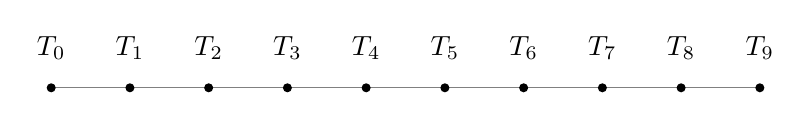
\begin{tikzpicture}
    \coordinate (Origin)   at (0,0);
    \coordinate (XAxisMin) at (0,0);
    \coordinate (XAxisMax) at (9,0);
    \draw [thin, gray] (XAxisMin) -- (XAxisMax);% Draw x axis
    \foreach \x in {0,1,...,9}{% Two indices running over each
        \node[draw,circle,inner sep=1pt,fill] at (\x,0) {};
    }
    \foreach \x in {0,1,...,9}{% Two indices running over each        
        \node [] at (\x, 0.5)  {$T_{\x}$};        
    }    
\end{tikzpicture}
\end{center}
\vfill 
What we need is a way to {\it decompose} this mesh so that
several processes can do the work.

\end{frame}


%------------------------------------------------------------------------------%
\begin{frame}{Another Application: Domain Decomposition}

For three processes, the mesh can be divided up as follows:

\begin{center}
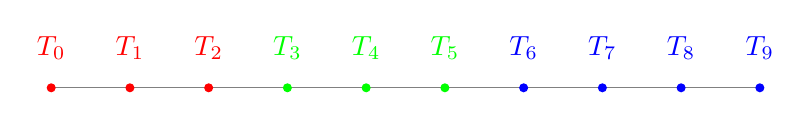
\begin{tikzpicture}
    \coordinate (Origin)   at (0,0);
    \coordinate (XAxisMin) at (0,0);
    \coordinate (XAxisMax) at (9,0);
    \draw [thin, gray] (XAxisMin) -- (XAxisMax);% Draw x axis
    \foreach \x in {0,1,...,2}{% Two indices running over each
        \node[red,draw,circle,inner sep=1pt,fill] at (\x,0) {};
    }
    \foreach \x in {0,1,...,2}{% Two indices running over each        
        \node [red] at (\x, 0.5)  {$T_{\x}$};        
    } 
    \foreach \x in {3,4,...,5}{% Two indices running over each
        \node[green,draw,circle,inner sep=1pt,fill] at (\x,0) {};
    }
    \foreach \x in {3,4,...,5}{% Two indices running over each        
        \node [green] at (\x, 0.5)  {$T_{\x}$};        
    }    
    \foreach \x in {6,7,...,9}{% Two indices running over each
        \node[blue,draw,circle,inner sep=1pt,fill] at (\x,0) {};
    }
    \foreach \x in {6,7,...,9}{% Two indices running over each        
        \node [blue] at (\x, 0.5)  {$T_{\x}$};        
    }       
\end{tikzpicture}
\end{center}
Consider $T_2$. The finite difference equation 
indicates that process 0 needs the value of $T_3$ to 
update $T_2$, but \textcolor{green}{process 1 is in charge of $T_3$}!  

\vfill 

Options:
\begin{enumerate}
 \item Each process has a full $T$ array and 
       communicates it to neighbors after each iteration.
 \item Each process has an array of size equal to the number of temperatures 
       it computes (here, 5), plus one or two extra ``ghost'' cells for 
       neighbor data.
\end{enumerate}

Option 1 is easy to code but (a) sends way too much data every time and
(b) requires more memory-per-process than is needed.  Option 2 is 
harder to code but minimizes communication and memory requirements. 
{\it We'll, of course, go with the second option.}

\end{frame}

%------------------------------------------------------------------------------%
\begin{frame}{Another Application: Domain Decomposition}

A schematic for decomposing the mesh and communicating
boundary information is shown below:

\begin{center}
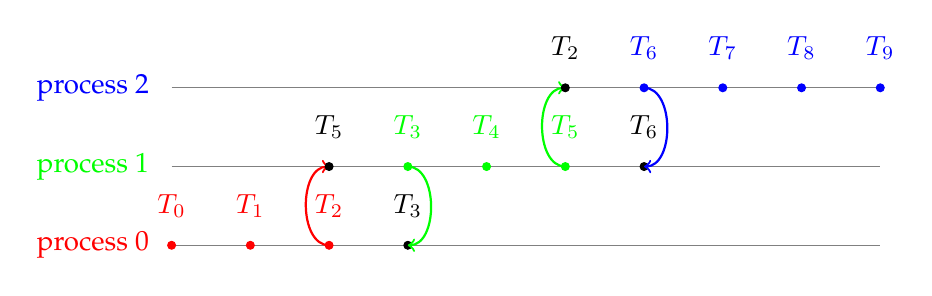
\begin{tikzpicture}
    \coordinate (Origin)   at (0,0);
    \coordinate (XAxisMin) at (0,0);
    \coordinate (XAxisMax) at (9,0);
    \draw [thin, gray] (0,0) -- (9,0);% Draw x axis
    \draw [thin, gray] (0,1) -- (9,1);% Draw x axis
    \draw [thin, gray] (0,2) -- (9,2);% Draw x axis
    \node [black] at (-1, 0)  {\textcolor{red}{process 0}};  
    \node [black] at (-1, 1)  {\textcolor{green}{process 1}};  
    \node [black] at (-1, 2)  {\textcolor{blue}{process 2}};  

    %---------------------------------------------------------------%
    \foreach \x in {0,1,...,2}{% Two indices running over each
        \node[red,draw,circle,inner sep=1pt,fill] at (\x,0) {};
    }
    \foreach \x in {0,1,...,2}{% Two indices running over each        
        \node [red] at (\x, 0.5)  {$T_{\x}$};        
    } 
    \node[black,draw,circle,inner sep=1pt,fill] at (3,0) {};
    \node [black] at (3, 0.5)  {$T_{3}$};   
    \path[draw]
      (2, 0) edge [red, bend left = 90, ->, thick] node [left] {} (2, 1);           
    %---------------------------------------------------------------%
    \foreach \x in {3,4,...,5}{% Two indices running over each
        \node[green,draw,circle,inner sep=1pt,fill] at (\x,1) {};
    }
    \foreach \x in {3,4,...,5}{% Two indices running over each        
        \node [green] at (\x, 1.5)  {$T_{\x}$};        
    }    
    \node[black,draw,circle,inner sep=1pt,fill] at (2,1) {};
    \node [black] at (2, 1.5)  {$T_{5}$};   
    \node[black,draw,circle,inner sep=1pt,fill] at (6,1) {};
    \node [black] at (6, 1.5)  {$T_{6}$};   
    \path[draw]
      (3, 1) edge [green, bend left = 90, ->, thick] node [left] {} (3, 0);    
    \path[draw]
      (5, 1) edge [green, bend left = 90, ->, thick] node [left] {} (5, 2);             
    %---------------------------------------------------------------%    
    \foreach \x in {6,7,...,9}{% Two indices running over each
        \node[blue,draw,circle,inner sep=1pt,fill] at (\x,2) {};
    }
    \foreach \x in {6,7,...,9}{% Two indices running over each        
        \node [blue] at (\x, 2.5)  {$T_{\x}$};        
    }    
    \node[black,draw,circle,inner sep=1pt,fill] at (5,2) {};
    \node [black] at (5, 2.5)  {$T_{2}$};  
    \path[draw]
      (6, 2) edge [blue, bend left = 90, ->, thick] node [left] {} (6, 1);     
    %---------------------------------------------------------------%    
    
\end{tikzpicture}
\end{center}
 
\vfill 

Therefore, each process but the last must send to its right, and
each process but the first must send to its left.
\vfill 
Likewise, each process but the last must receive from its right
neighbor, and each process but the first must receive from its
left neighbor.

\end{frame}

%------------------------------------------------------------------------------%
\begin{frame}{Handling Ghost Cells: a Python Snippet}


\lstinputlisting[language=Python]{ghost_cell_snippet.py}

where {\tt i\_s} and {\tt i\_e} are starting and ending indices
of the {\it local temperature array}.
For example, process 3 computes temperatures {\tt T[1:4]}
(where the local 1 and 4 map onto the global 3 and 6, respectively).  Then,
process 3 sends
{\tt T[1]} and {\tt T[3]} (globally, 
$T_3$ and $T_5$), and receives 
{\tt T[0]} and {\tt T[4]} (globally $T_2$ and $T_6$).

\vfill 

\textcolor{blue}{Exercise}: 
Switch the first two if statements and run your code with three 
processes.  What happens and why?  The phenomenon is called 
{\it deadlock} and is as common a bug for MPI programs as are 
race conditions in OpenMP programs.

\end{frame}

%------------------------------------------------------------------------------%
\begin{frame}{Hints for the Full Implementation}


\begin{itemize}
 \item Think carefully about how to handle (the physical) boundary conditions.
       Not all processes will have such a condition to handle.
 \item If you terminate the iteration when the difference of successive 
       temperatures is below some threshold $\tau$
       (e.g., $\max(|\mathbf{T} - \mathbf{T}^{\text{old}}|) < \tau$), then each
       process needs the same difference for comparison to a tolerance.  Otherwise,
       some processes might keep iterating, and your code will hang when 
       they try to send to and receive from processes no longer iterating.
 \item Ideally, you'll get the full, final temperature array onto the root 
       process for plotting and such.  You've seen a few functions for 
       doing this, but {\tt gather} might be a clean approach.
 \item In 2-D, you'll need whole rows of ghost cells, so think carefully about 
       your indices.
\end{itemize}


\end{frame}



\end{document}
